\section{An Unreliable Datagram Extension to QUIC}
\label{sec:datagrams}
QUIC is by default a reliable protocol.
However there are plenty of situations where transmission speed is more important than reliability, especially in real-time communication.
\textit{An Unreliable Datagram Extension to QUIC}~\cite{ietf-quic-datagram-02} introduces a new QUIC frame called DATAGRAM which carry data unreliably.

According to~\cite{ietf-quic-datagram-02} DATAGRAM frames are not retransmitted.
They are sent alongside the STREAM frames so they use the same cryptography context but they don't affect flow-control limits.
Each DATAGRAM frame is acknowledged so it is possible to provide application with information about packet loss.
It is also important that DATAGRAM frames are subject to QUIC congestion control mechanism which allows applications to avoid implementing their own.

Number of experiments have been performed to validate DATAGRAM frames behavior as well as their ease of use.
They are presented in the following sections.

\subsection{Test environment}
\label{subsec:test-env}
Figure~\ref{fig:dgram_test_env} shows test environment used in DATAGRAM frames experiments.
Both machines are in local network.

\begin{figure}
    \centering
    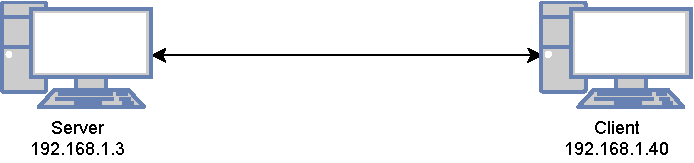
\includegraphics[width=0.8\textwidth]{img/__09__datagrams/dgram_test_env.pdf}
    \caption{Test environment}
    \label{fig:dgram_test_env}
\end{figure}

\subsection{Flow control}
\label{subsec:flow-control}
As stated above DATAGRAM frames are not subject to flow control mechanism.
Thanks to this we can limit data that can be sent in a reliable way to allow for better unreliable communication.

\subsubsection{Tests}
This test illustrates DATAGRAM frames behavior in case of reaching flow control limit on any of streams used in the connection.
Test environment was described in~\ref{subsec:test-env}.
Client opens two bidirectional streams while server sets their flow control limit to 1000B\@.
In each iteration client tries to send 10 reliable and 10 unreliable messages of size 800B each.
Figure~\ref{fig:dgram_flow_control} presents this scenario.

\begin{figure}
    \centering
    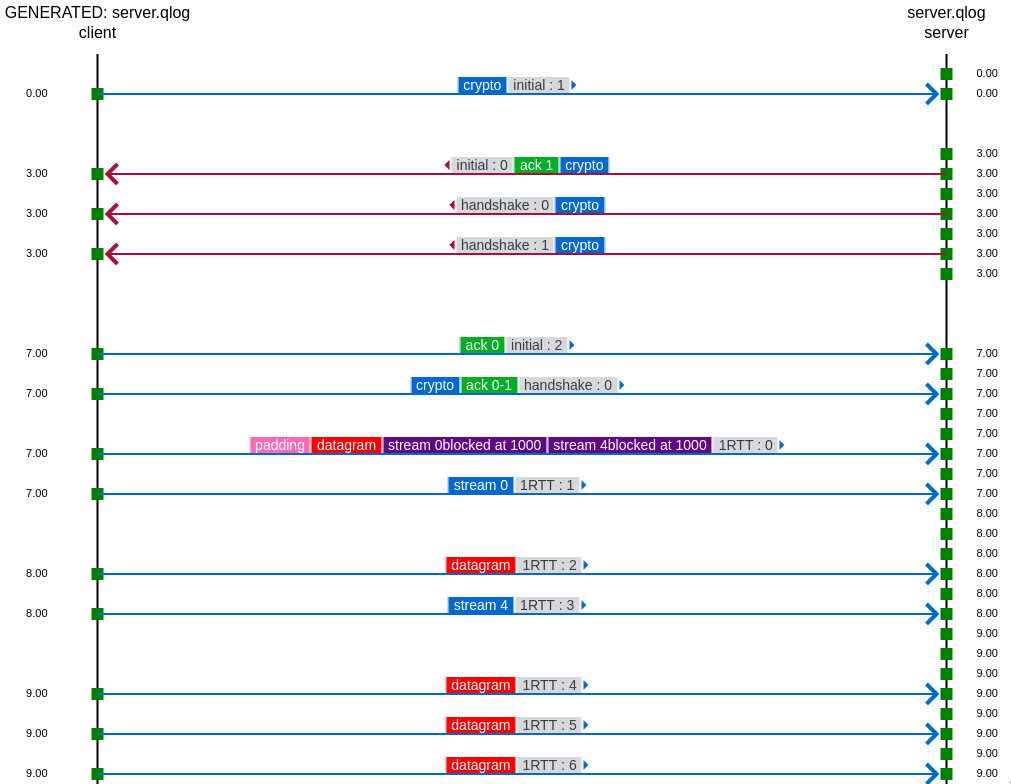
\includegraphics[width=\textwidth]{img/__09__datagrams/dgram_flow_control.png}
    \caption{DATAGRAM flow control test}
    \label{fig:dgram_flow_control}
\end{figure}

After establishing the connection client starts sending data.
He sends two 1-RTT packets with STREAM frames (packets 1 and 3) and reaches flow control limit.
However, he is still able to send packets with DATAGRAM frames (packets 4, 5, 6).

% \begin{figure}[h]
%   \centering
%   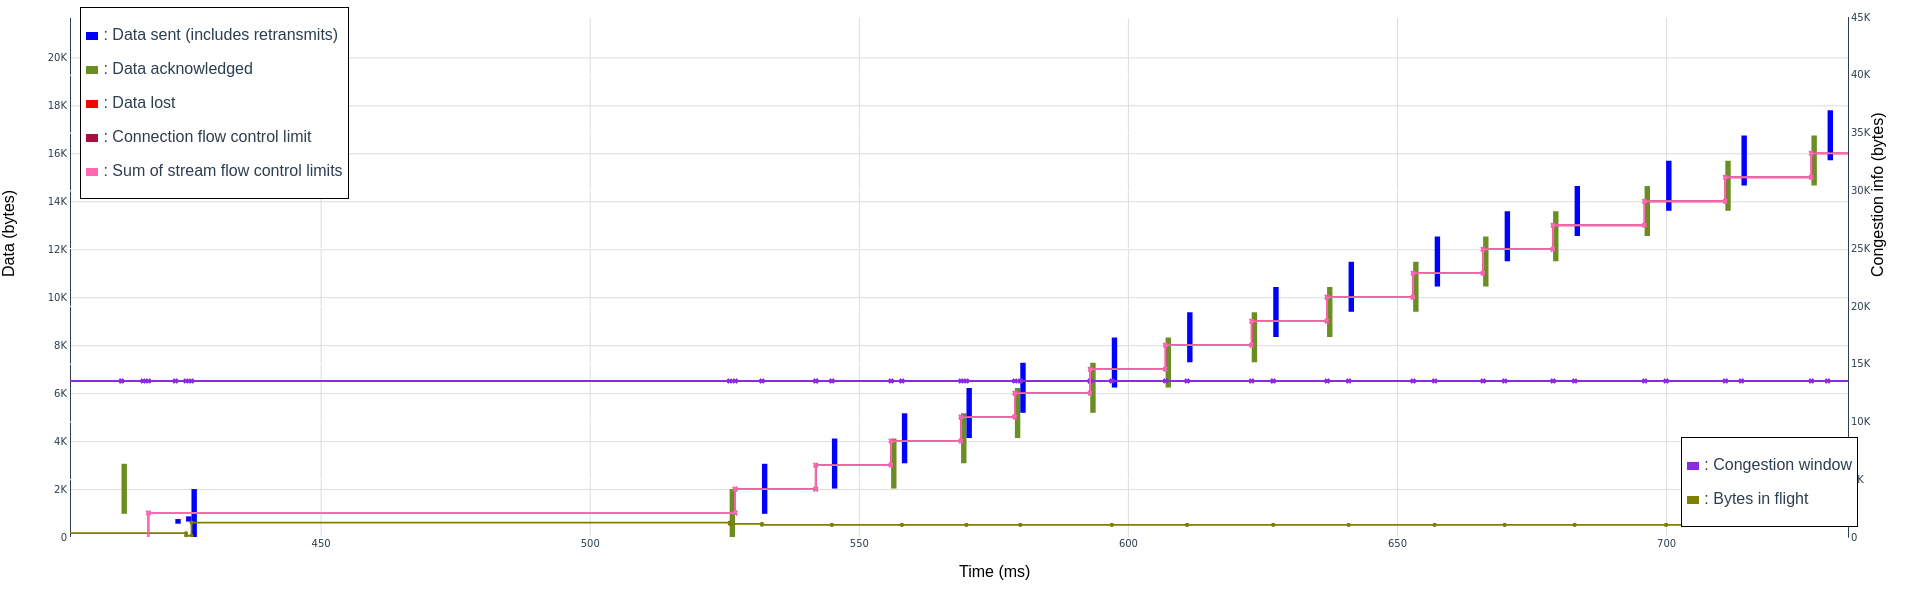
\includegraphics[width=\textwidth]{img/__09__datagrams/stream_flow_control_2.png}
%   \caption{DATAGRAM flow control test}
%   \label{fig:stream_flow_control2}
% \end{figure}

Figure~\ref{fig:dgram_flow_control2} shows this behavior from different perspective.
\begin{figure}
    \centering
    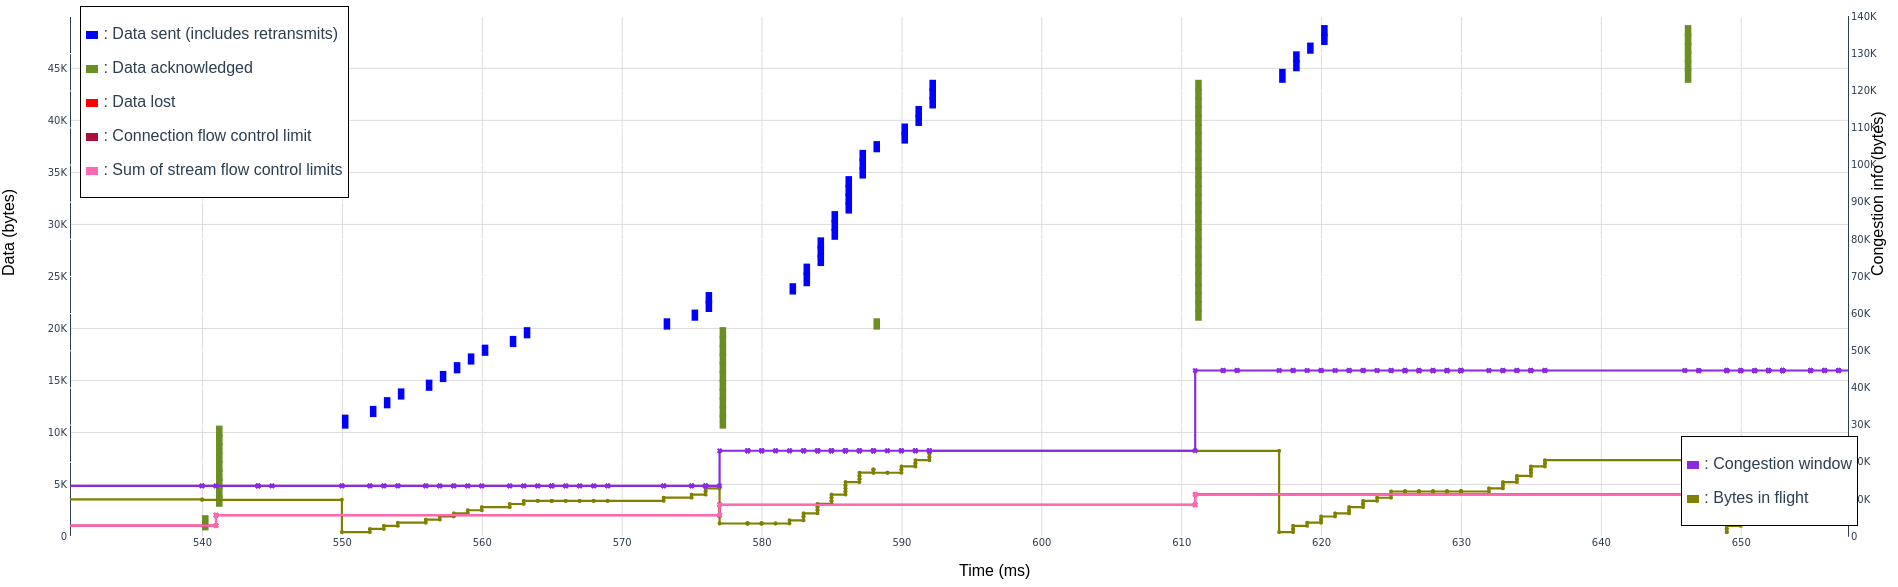
\includegraphics[width=\textwidth]{img/__09__datagrams/dgram_flow_control_2.png}
    \caption{DATAGRAM flow control test}
    \label{fig:dgram_flow_control2}
\end{figure}
Pink line indicates sum of stream flow control limit whereas blue bars represent data sent.
We can see that despite the fact flow control limit is less than 5kB we send much more data -- over 45kB\@.

\subsection{Loss detection}
\label{subsec:loss-detection}
From RFC 9002 (Section 6.1), a packet is declared lost if it meets all of the following conditions:
\begin{itemize}
    \item The packet is unacknowledged, in flight, and was sent prior to an acknowledged packet.
    \item The packet was sent kPacketThreshold packets before an acknowledged packet (Section 6.1.1), or it was sent long enough in the past (Section 6.1.2)~\cite{rfc9002}.
\end{itemize}

What is important is that to consider packet is lost there has to be some other packet that was sent later and has already been acknowledged.

\subsubsection{PTO}
A Probe Timeout (PTO) triggers the sending of one or two probe datagrams when ack-eliciting packets are not acknowledged within the expected period of time or the server may not have validated the client's address.
A PTO enables a connection to recover from loss of tail packets or acknowledgments~\cite{rfc9002} (RFC 9002, Section 6.2).

Expiration of PTO timer does not indicate the packet was lost.
It only provides one of the requirements necessary to consider the packet as lost -- the packet was sent prior to an acknowledged packet.
PTO timer is reset each time a new ack-eliciting packet was sent or received.

\subsubsection{Tests}
This test illustrates the impact of packet loss on communication with DATAGRAM frames.
Test environment was described in~\ref{subsec:test-env}.
Additionally, in some scenarios client machine had some packet loss set for all UDP datagrams which destination port was equal to 4433.
This was done using Linux TC software.

The test consists of three scenarios.
In each scenario client was trying to send 1000 messages of 500B size each.
Server responsibility was to respond for each message by returning it back to the client.
After sending each message client was waiting for the response from the sever specified amount of time.
The summary is presented in table~\ref{tab:dgram_packet_loss}.

\begin{table}
    \centering
    \resizebox{\columnwidth}{!}{%
    \begin{tabular}{|c | c | c | c | c | c |}
        \hline
        \multicolumn{2}{|c}{\makecell{0\% packet loss}} & \multicolumn{2}{|c}{\makecell{10\% packet loss}} & \multicolumn{2}{|c|}{\makecell{30\% packet loss}} \\
        \hline
        \multicolumn{2}{|c}{client} & \multicolumn{2}{|c|}{client} & \multicolumn{2}{|c|}{client} \\
        \hline
        packets sent & packets lost & packets sent & packets lost & packets sent & packets lost \\
        \hline
        1005         & 0            & 1007         & 89           & 1031         & 318          \\
        \hline
    \end{tabular}%
    }
    \caption{\label{tab:dgram_packet_loss}Number of packets sent with and without packet loss for DATAGRAM frames.}
\end{table}

In the first scenario messages were sent via DATAGRAM frames without packet loss.
As a result client sent 1005 packets.
None of them were lost.

In the second scenario messages were sent via DATAGRAM frames but packet loss was set to 10\%.
As a result client sent 1007 packets, 89 of which were lost.
We can see that in this scenario client sent 2 packets more than in the first scenario.
This is because server sends its data as last and client need to acknowledge this data by sending additional packet with ACK frame but it is not important.

In the last scenario, messages were sent via DATAGRAM frames but packet loss was set to 30\%.
As a result client sent 1031 packets, 318 of which were lost.
This time we can observe that client sent ~20-30 packets more than in the first two scenarios.
It's because of PING frames that are being sent when PTO timer expires.
Figure~\ref{fig:dgram_ping_frames} illustrates this situation.

\begin{figure}
    \centering
    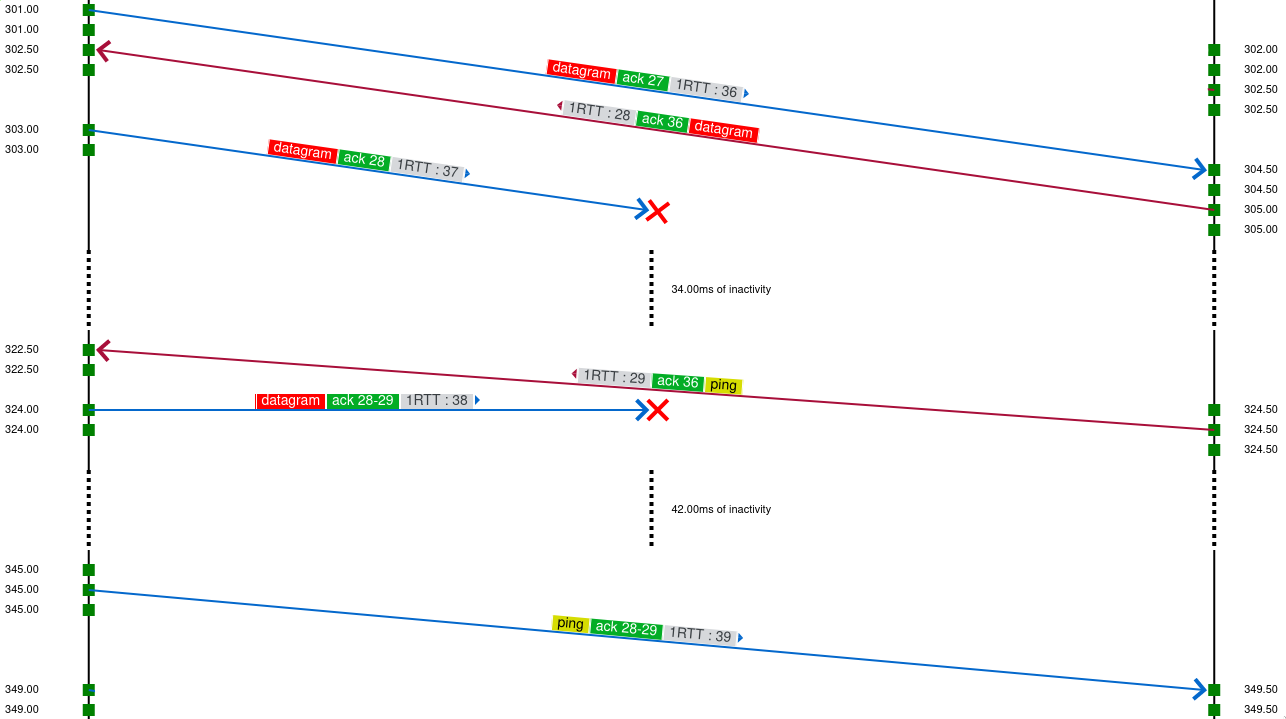
\includegraphics[width=\textwidth]{img/__09__datagrams/dgram_retransmission_ping.png}
    \caption{Sending PING frame after server or client inactivity.
    Client messages are described by blue arrows.
    Numbers on the left and right side indicate time in ms when given packet was sent or received.}
    \label{fig:dgram_ping_frames}
\end{figure}

Server in its 28th 1RTT packet sent datagram frame in response to client's earlier packet and set its PTO timer.
Client received server's packet, generated a response and set its own timer.
The response was lost so that server's PTO timer expired which resulted in 29th 1RTT packet from server to client with PING frame.
After receiving it client generated a response, reset its PTO timer and sent the response but this time it was also lost.
After 21 ms client's PTO timer expired so client sent a new ack-eliciting packet with PING frame.
